\documentclass[final]{lmuposter}
%\usepackage[utf8x]{inputenc}
\usepackage[T1]{fontenc}
%\usepackage[scaled]{beramono}
\usepackage{lmodern}
\usepackage{tikz}
\usepackage{amsmath}
\usepackage{tabularx}
\usepackage{amssymb}
\usepackage{bbm}
%\usepackage{paralist}
\usepackage{verbatim}
\usepackage{multicol}
\usepackage{wallpaper}


% Python listing setup

\usepackage{color}
\usepackage[procnames]{listings}
\usepackage{textcomp}
\usepackage{setspace}
\usepackage[]{xcolor}
\definecolor{gray}{gray}{0.5}
\definecolor{green}{rgb}{0,0.5,0}
\definecolor{lightgreen}{rgb}{0,0.7,0}
\definecolor{purple}{rgb}{0.5,0,0.5}
\definecolor{darkred}{rgb}{0.7,0,0}

\lstnewenvironment{python}[1][]{
\lstset{
% Escape with funnyeyes.
escapeinside={(*@}{@*)},
language=python,
basicstyle=\ttfamily\small,
stringstyle=\color{green},
showstringspaces=false,
alsoletter={1234567890},
otherkeywords={\ , \}, \{},
keywordstyle=\color{blue},
emph={access,and,as,break,class,continue,def,del,elif,else,%
except,exec,finally,for,from,global,if,import,in, is,%
lambda,not,or,pass,print,raise,return,try,while,assert},
emphstyle=\color{orange}\bfseries,
emph={[2]self},
emphstyle=[2]\color{gray},
emph={[4]ArithmeticError,AssertionError,AttributeError,BaseException,%
DeprecationWarning,EOFError,Ellipsis,EnvironmentError,Exception,%
False,FloatingPointError,FutureWarning,GeneratorExit,IOError,%
ImportError,ImportWarning,IndentationError,IndexError,KeyError,%
KeyboardInterrupt,LookupError,MemoryError,NameError,None,%
NotImplemented,NotImplementedError,OSError,OverflowError,%
PendingDeprecationWarning,ReferenceError,RuntimeError,RuntimeWarning,%
StandardError,StopIteration,SyntaxError,SyntaxWarning,SystemError,%
SystemExit,TabError,True,TypeError,UnboundLocalError,UnicodeDecodeError,%
UnicodeEncodeError,UnicodeError,UnicodeTranslateError,UnicodeWarning,%
UserWarning,ValueError,Warning,ZeroDivisionError,abs,all,any,apply,%
basestring,bool,buffer,callable,chr,classmethod,cmp,coerce,compile,%
complex,copyright,credits,delattr,dict,dir,divmod,enumerate,eval,%
execfile,exit,file,filter,float,frozenset,getattr,globals,hasattr,%
hash,help,hex,id,input,int,intern,isinstance,issubclass,iter,len,%
license,list,locals,long,map,max,min,object,oct,open,ord,pow,property,%
quit,range,raw_input,reduce,reload,repr,reversed,round,set,setattr,%
slice,sorted,staticmethod,str,sum,super,tuple,type,unichr,unicode,%
vars,xrange,zip},
emphstyle=[4]\color{purple}\bfseries,
upquote=true,
morecomment=[s][\color{lightgreen}]{"""}{"""},
commentstyle=\color{red}\slshape,
literate={>>>}{\bfseries{\textcolor{darkred}{>{>}>}}}3%
         {...}{{\textcolor{gray}{...}}}3,
procnamekeys={def,class},
procnamestyle=\color{blue}\textbf,
framexleftmargin=1mm, framextopmargin=1mm,
rulesepcolor=\color{blue},#1
}}{}


%% -----------------------------------------------------------------------------
%
%\newtheorem{definition}{Definition}
\newcommand{\foot}[1]{_{\mbox{\footnotesize #1}}}
\newcommand{\head}[1]{^{\mbox{\footnotesize #1}}}
%
%
\newcommand{\ones}{\mathbb{I}}
\newcommand{\nat}{\mathbb{N}}
\newcommand{\real}{\mathbb{R}}
\newcommand{\ganz}{\mathbb{Z}}
%
%
\newcommand{\RRE}{\mbox{RRE}}
\newcommand{\nnz}[1]{\mbox{nnz}(#1)}
\newlength{\Hoehe}
\renewcommand{\vec}[1]{#1}
\newlength{\GLaenge}
\setlength{\GLaenge}{3.5cm}
%
%
\definecolor{MyGrey}{gray}{0.45}
\def\bstheta{\boldsymbol{\theta}}
\def\bsalpha{\boldsymbol{\alpha}}
\def\bsk{\boldsymbol{k}}
\def\bsx{\boldsymbol{x}}
\def\bsh{\boldsymbol{h}}
%
% Centred minipage environment
%
\newenvironment{cmpage}[1]{
\begin{center}
\begin{minipage}{#1\textwidth}}%
{\end{minipage}\end{center}}
%
%
\newcommand{\POS}{\color{blue}\item [\boldmath{$+$}]}
\newcommand{\NEG}{\color{red}\item [{\boldmath$-$}]}
\newcommand{\NTR}{\color{black}\item [$\circ$]}
\newcommand{\f}[1]{\mathfrak{#1}}
\newcommand{\old}{^{\mbox{\small \color{blue} old}}}
\newcommand{\new}{^{\mbox{\small \color{red} new}}}
\newcommand{\diag}[1]{\mbox{diag}\left(#1\right)}
%
%
\newcommand{\myBlank}{\textvisiblespace}
\newcommand{\noSpace}{\makebox[0pt]{\quad}}
%
% Old style colour commands
%
\newcommand{\CB}{\color{blue}}
\newcommand{\CR}{\color{red}}
\newcommand{\CG}{\color{green}}
\newcommand{\CC}{\color{cyan}}
%
\definecolor{myWhite}{rgb}{1.00,1.00,1.00}  % real white
\definecolor{myGrey}{rgb}{0.78,0.83,0.94}   % 'light grey blue'
\definecolor{myYellow}{rgb}{1.00,1.00,0.00} % yellow
\definecolor{myOrange}{rgb}{1.00,0.65,0.00} % orange
\definecolor{myCyan}{rgb}{0.00,1.00,1.00}   % cyan
%
% Some abbrevs for setting brief code parts
%
\newcommand{\ttA}{\mbox{\texttt{A}}}
\newcommand{\ttB}{\mbox{\texttt{B}}}
\newcommand{\ttC}{\mbox{\texttt{C}}}
\newcommand{\ttD}{\mbox{\texttt{D}}}
\newcommand{\code}[1]{\mbox{\texttt{#1}}}
\newcommand{\ccode}[1]{\cemphd{\texttt{#1}}}
%
% Commands for slides taken from 'Insides'
%
\newcommand{\rst}{\textcolor{emphcolora}{\ast}}
\newcommand{\bst}{\textcolor{emphcolorb}{\ast}}
%
%
%
\definecolor{textcolor} {rgb}{0,0,0}
\definecolor{decocolor} {rgb}{0,0,0}
\definecolor{emphcolora}{rgb}{1,0,0}              % pure red
\definecolor{emphcolorb}{rgb}{0,0,1}              % pure blue
\definecolor{emphcolorc}{cmyk}{0,1,0,0}           % pure magenta
%\definecolor{emphcolord}{cmyk}{0.64,0,0.95,0.20} % sort of green
\definecolor{emphcolord}{rgb}{0,0.4,0.12}         % same as lmu@darkgreen
\definecolor{emphcolore}{cmyk}{1,0,0,0}           % pure cyan
\definecolor{linkcolor} {rgb}{0,0,0}
%
% Commands emphasising text using color
%
\newcommand{\cempha}[1]{{\color{emphcolora}#1}}
\newcommand{\cemphb}[1]{{\color{emphcolorb}#1}}
\newcommand{\cemphc}[1]{{\color{emphcolorc}#1}}
\newcommand{\cemphd}[1]{{\color{emphcolord}#1}}
\newcommand{\cemphe}[1]{{\color{emphcolore}#1}}
\newcommand{\cemphf}[1]{{\color{decocolor}#1}}
% -----------------------------------------------------------------------------
% myColorBox
% -----------------------------------------------------------------------------
\setbeamercolor{myBoxColor}{fg=black,bg=white}
\setbeamercolor{myBoxColorHead}{fg=red,bg=white}
% \newenvironment{myColorBox}[2]{%
% \begin{beamerboxesrounded}[shadow=true,lower=myBoxColor,upper=myBoxColorHead,
% width=#1\textwidth]{#2}}%
% {\end{beamerboxesrounded}}
\newenvironment{myColorBox}[2]{%
\begin{cmpage}{#1}%
\begin{beamerboxesrounded}[shadow=true,lower=myBoxColor,upper=myBoxColorHead]%
{#2}}%
{\end{beamerboxesrounded}\end{cmpage}}
%
% -----------------------------------------------------------------------------
% Math Operators, alternate greek symbols and the like
% -----------------------------------------------------------------------------
\DeclareMathOperator{\grad}{grad}
\DeclareMathOperator{\mydiv}{div}
\DeclareMathOperator{\Grad}{grad}
\DeclareMathOperator{\Div}{div}
%\newcommand{\grad}{\mbox{grad}}
%\newcommand{\mydiv}{\mbox{div}}
\renewcommand{\rho}{\varrho}
%
% -----------------------------------------------------------------------------
% Some color defintions to be compatible with XFIG
% -----------------------------------------------------------------------------
%
\definecolor{XFIGgold}{rgb}{1.00,0.84,0.00}
\definecolor{XFIGltblue}{rgb}{0.53,0.81,1.00}
\definecolor{XFIGred}{rgb}{1.00,0.00,0.00}
% -----------------------------------------------------------------------------


\usepackage{fontspec}
\defaultfontfeatures{Mapping=tex-text}
\setmainfont{Helvetica}


\setlength{\parindent}{0pt}
\setlength{\itemsep}{1mm}
\setlength{\parsep}{1mm}
\renewcommand{\labelitemi}{\footnotesize $\bigstar$}
\renewcommand{\labelitemii}{\footnotesize $\blacktriangleright$}
\newcommand{\capsize}{\small}

\begin{document}

%\TileWallPaper{5cm}{5cm}{./noisy_grid/noisy_grid_@2X.png}
\TileWallPaper{5cm}{5cm}{./honey_im_subtle/honey_im_subtle_@2X.png}

\PosterHead{\textbf{\LARGE \huge ObsPy: A Python Toolbox for Seismology and Seismological Observatories}\\[0.5ex]
\large Lion Krischer$^1$, Tobias Megies$^1$, Robert Barsch$^2$, Moritz Beyreuther, Joachim Wassermann$^1$, and The ObsPy Development Team\\
$^1$ Department of Earth and Environmental Sciences, Ludwig-Maximilians-Universität München \\
$^2$ EGU Office \\
Contact:\hspace{0.6cm} \textit{devs@obspy.org}\hspace{0.6cm} \textbf{http://www.obspy.org}}



\vspace{-4ex}

\setlength{\columnsep}{\MyBoxHSep}
\begin{multicols}{3}


\MyBox[8em]{
\section*{Summary}

\textbf{Python} combines the power of a \textbf{full-blown programming language} with the
flexibility and accessibility of an \textbf{interactive scripting language}. Its
extensive standard library and large variety of freely available high quality
scientific modules cover most needs in developing \textbf{scientific processing
workflows}.

\textbf{ObsPy extends Python’s capabilities to fit the specific needs that
arise when working with seismological data.} It a) comes with a continuously
growing \textbf{signal processing toolbox} that covers most tasks common in
seismological analysis, b) provides \textbf{read and write support for many
common waveform, station and event metadata formats} and c) enables
\textbf{access to various data centers, webservices and databases} to retrieve
waveform data and station/event metadata.

In combination with mature and free Python packages like \textbf{NumPy},
\textbf{SciPy}, \textbf{Matplotlib}, \textbf{IPython}, \textbf{Pandas},
\textbf{lxml}, and \textbf{PyQt}, ObsPy makes it possible to develop complete
workflows in Python, ranging from reading locally stored data or requesting
data from one or more different data centers via signal analysis and data
processing to visualization in GUI and web applications, output of
modified/derived data and the creation of publication-quality figures.

All functionality is \textbf{extensively documented} and the \textbf{ObsPy
Tutorial} and Gallery give a good impression of the wide range of possible use
cases. ObsPy is tested and \textbf{running on Linux, OS X and Windows} and
comes with installation routines for these systems. ObsPy is developed in a
test-driven approach and is available under the \textbf{LGPLv3 open source
licence}.

Users are welcome to request help, report bugs, propose enhancements or
contribute code via either the user mailing list or the \textbf{project page on
GitHub}.

}
\vspace{\MyBoxVSep}


\MyBox[8em]{
\section*{Why Python?}
    \begin{itemize}
        \item Easy to learn $\Rightarrow$ Learning curve similar to Matlab
        \item Free and  Open Source
        \item Cross-platform $\Rightarrow$ Runs everywhere from Raspberry Pis to large supercomputers
        \item General purpose language (in contrast to many other tools used in science)
        \item No need to compile and interactive shell available
        \item ``Batteries included''
        \item Mature third party libraries
        \item Makes it easy to interact with existing C and Fortran code

        \item One of the most used programming languages
        \item Huge community outside of science $\Rightarrow$ Tools and support widely available
        \item Used a lot in the web community $\Rightarrow$ Will become more and more important
        \item Big support from the data analysis community
        \item Interesting new developments: PyPy, Blaze, numba, IPython, pandas, \dots
    \end{itemize}
    \vspace{0.245em}
}
\vspace{\MyBoxVSep}

\setlength{\MyBoxWidth}{714mm}

\MyBox[11.6em]{
    \vspace{1ex}

    \begin{tabularx}{\textwidth}{XXXXXX}

        \begin{minipage}{0.3\columnwidth}
            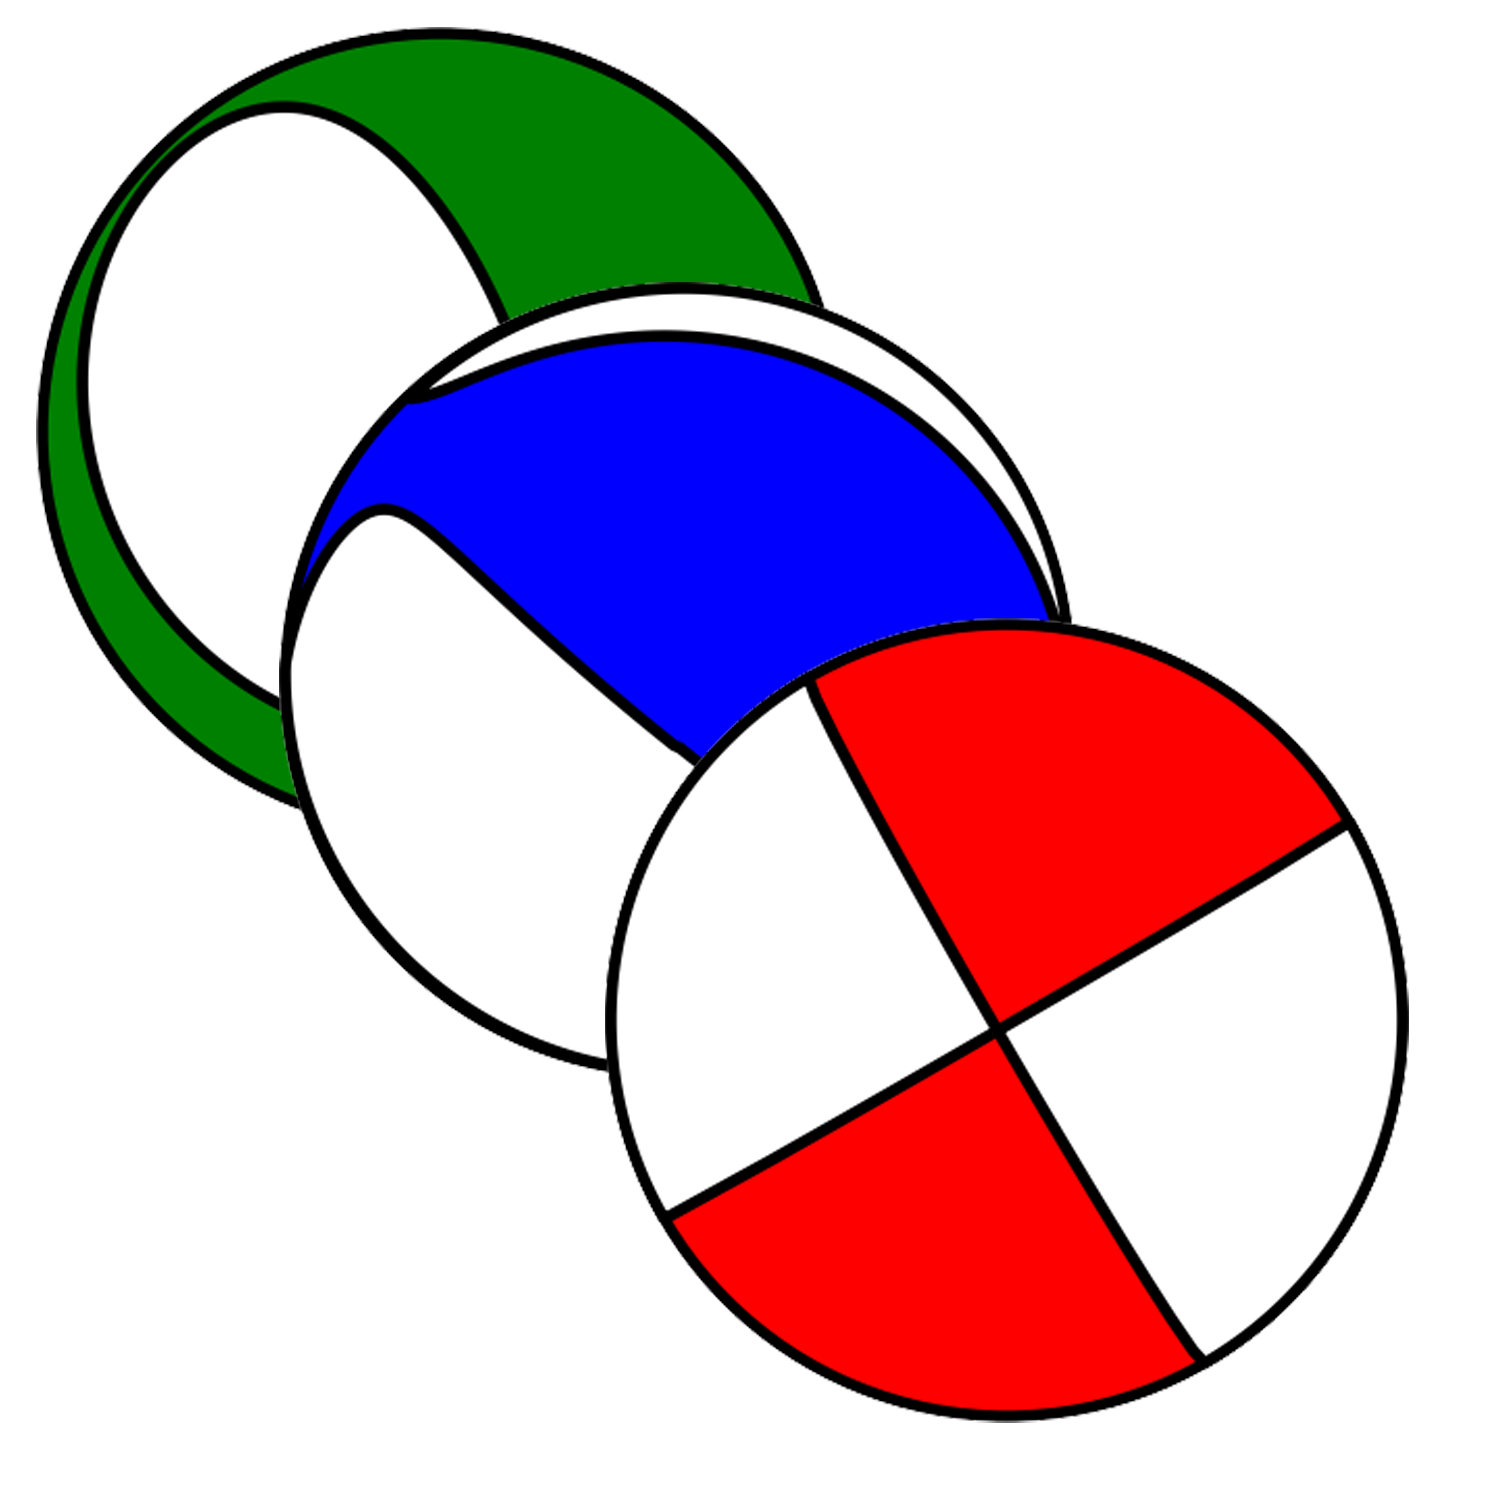
\includegraphics[height=10.6em]{image5.png}
        \end{minipage}
        &
        \hspace{-3ex}
        \begin{minipage}{0.3\columnwidth}
            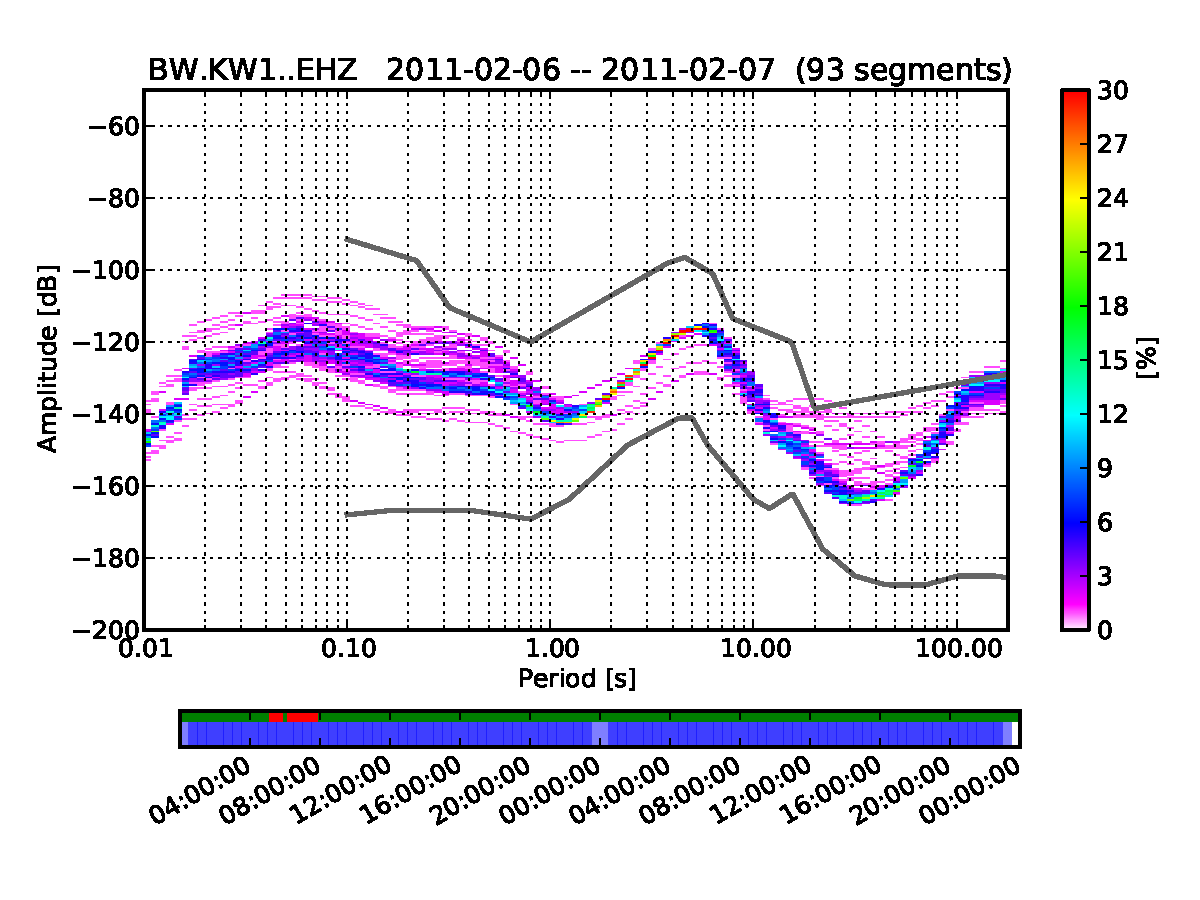
\includegraphics[height=10.6em]{image3.pdf}
        \end{minipage}
        &
        \begin{minipage}{0.3\columnwidth}
            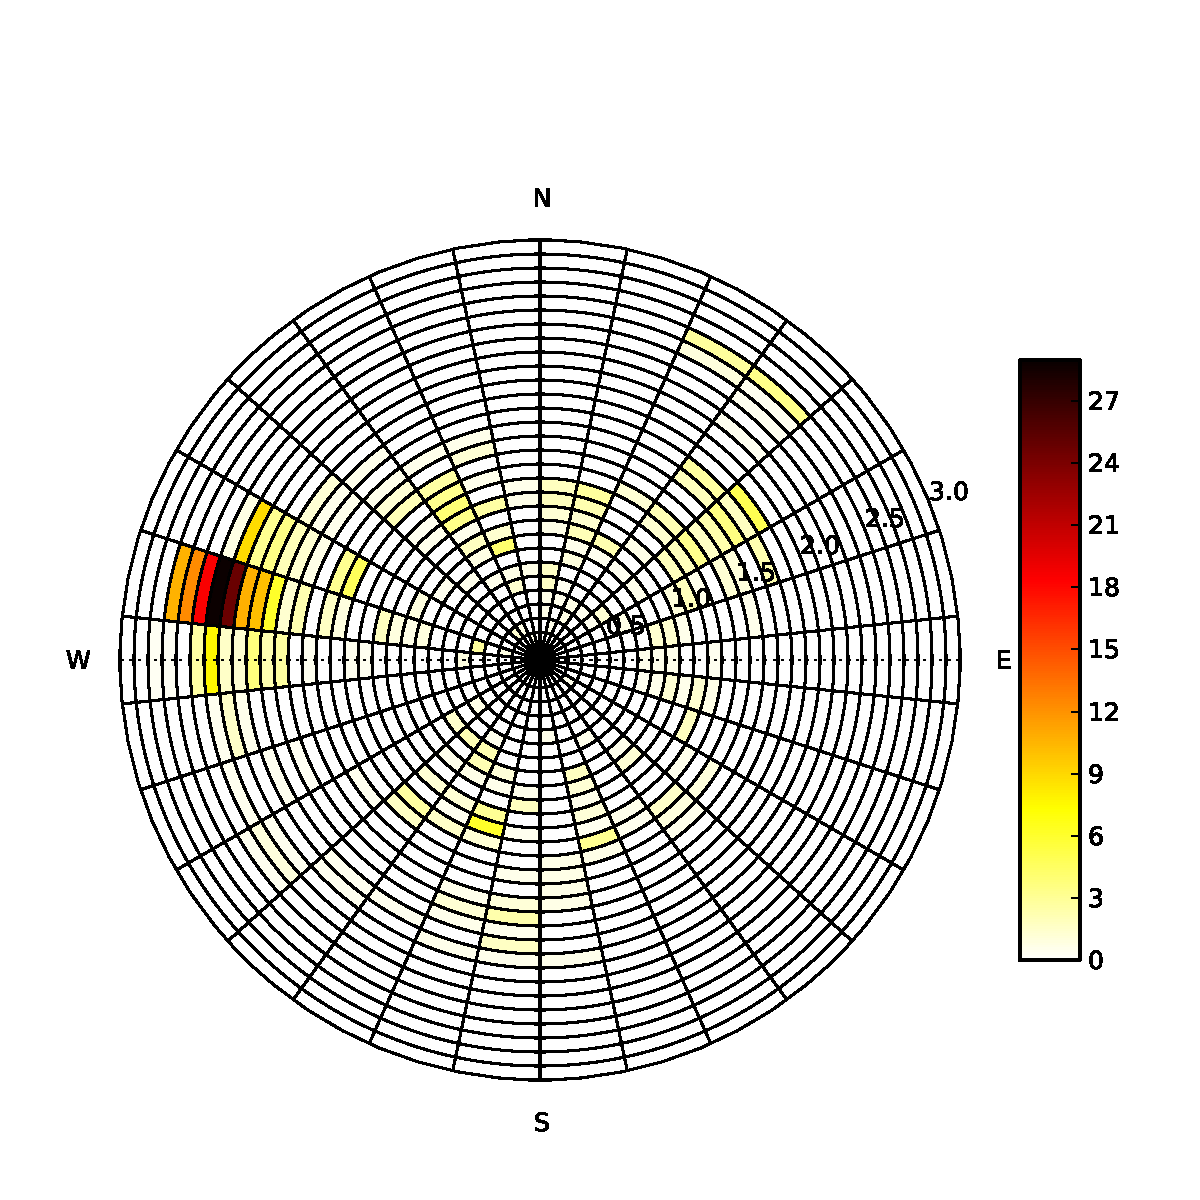
\includegraphics[height=10.6em]{image2.pdf}
        \end{minipage}
        &
        \begin{minipage}{0.3\columnwidth}
            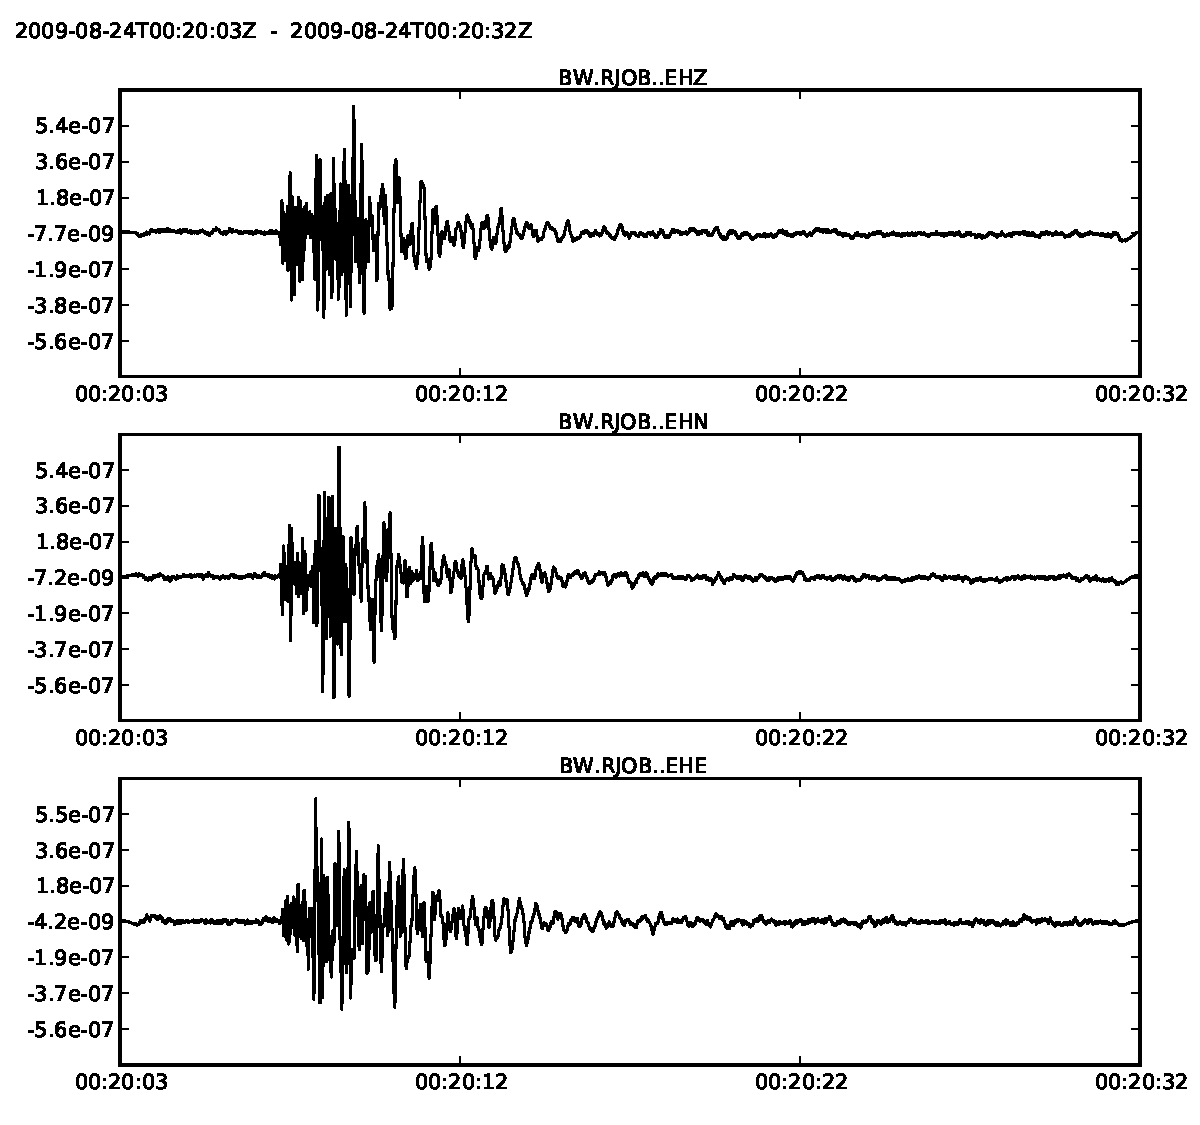
\includegraphics[height=10.6em]{image1.pdf}
        \end{minipage}
        &
        \begin{minipage}{0.3\columnwidth}
            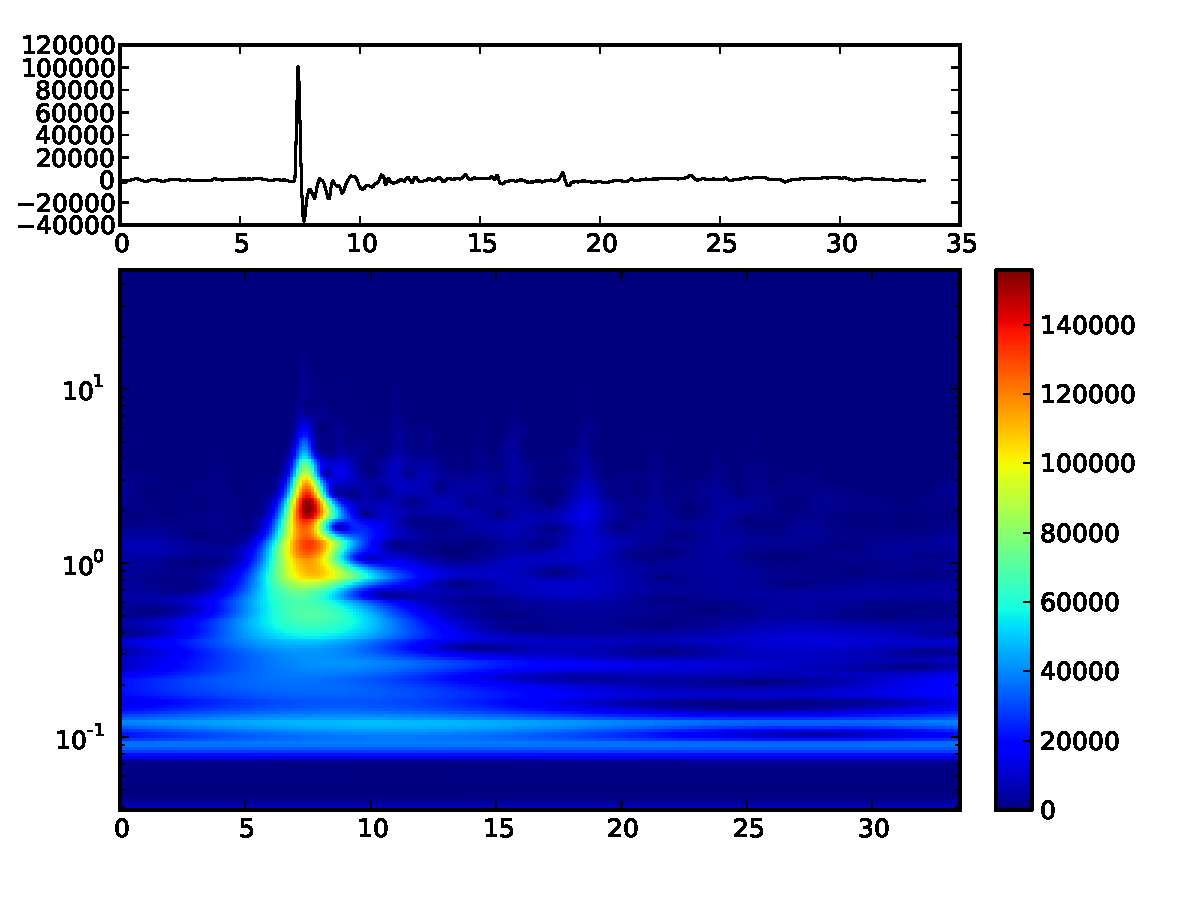
\includegraphics[height=10.6em]{image4.pdf}
        \end{minipage}
        &
        \begin{minipage}{0.3\columnwidth}
            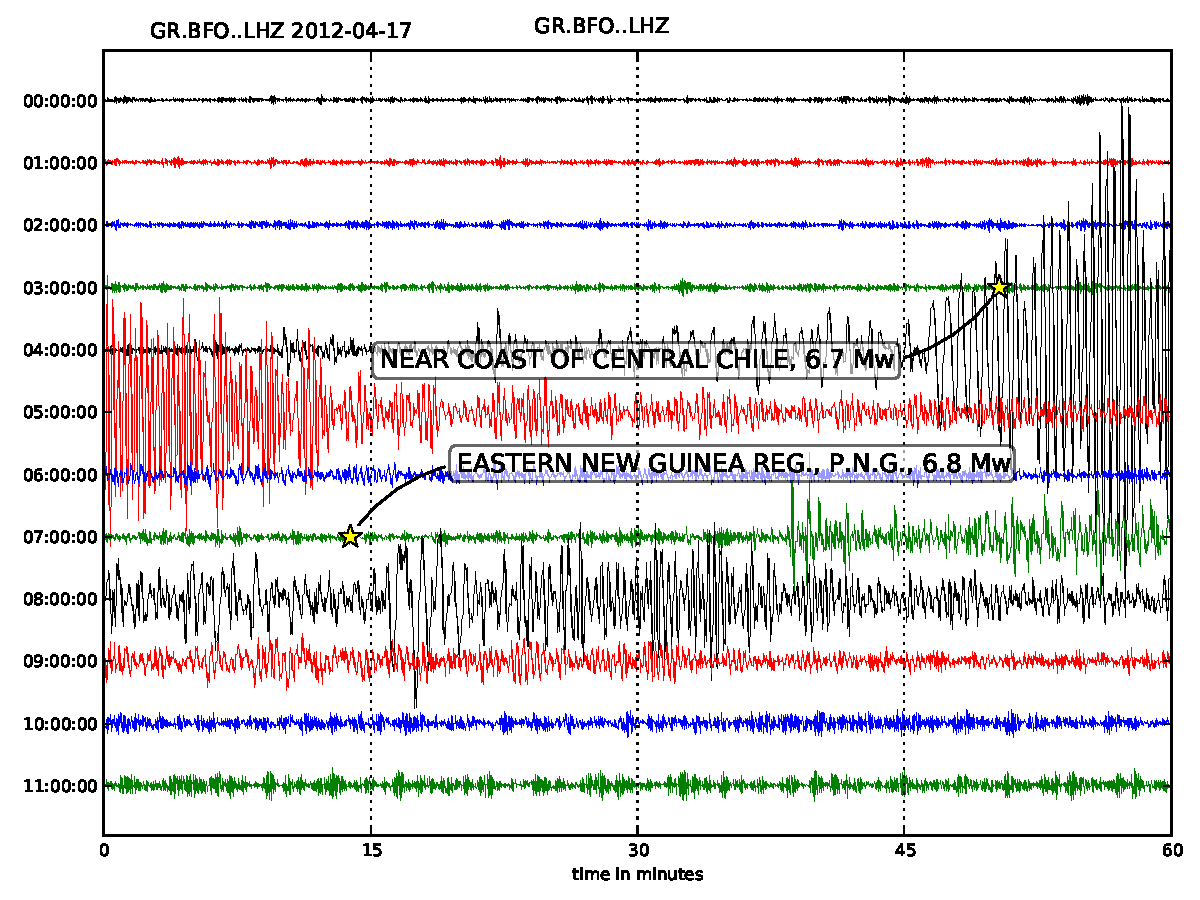
\includegraphics[height=10.6em]{image6.pdf}
        \end{minipage}\hspace{3ex}

    \end{tabularx}\hspace{3ex}
}

\setlength{\MyBoxWidth}{343mm}

\columnbreak




\MyBox[8em]{
\section*{What Can ObsPy Do?}
    \begin{itemize}
        \item \textbf{Read and write waveform data in various formats} (MiniSEED, SAC, GSE, SEG Y, \dots) with a unified interface.
        \item \textbf{Database and webservice access clients} for NERIES, IRIS DMC, ArcLink, SeisHub and Earthworm (experimental).
        \item \textbf{Many seismological signal processing routines} like filters, trigger, instrument correction, array analysis, beamforming, \dots
        \item \textbf{Support for inventory data} (SEED, XSEED, RESP and planned StationXML support)
        \item \textbf{Event data handling} (Supports the latest QuakeML 1.2 version)
        \item \textbf{Unified time handling} Uses UTC $\Rightarrow$ No ambiguities
    \end{itemize}
    \begin{center}
        +
    \end{center}

    \begin{center}
        \textbf{The full power and flexibility of Python.}
    \end{center}
}
\vspace{\MyBoxVSep}


\MyBox[8em]{
\section*{Example}
\begin{center}
\begin{minipage}{\columnwidth}
\begin{python}^^J
>>> from obspy import read^^J
>>> st = read("waveform.mseed")^^J
>>> print st^^J
1 Trace(s) in Stream:^^J
BW.FURT..EHZ | 2010-01-04 ... | 200.0 Hz, 7204234 samples^^J
>>> st[0].data^^J
array([-426, -400, ... , -489, -339], dtype=int32)^^J
>>> st.trim(endtime=st[0].stats.starttime + 3600)^^J
>>> st.decimate(factor=2)^^J
>>> st.filter("lowpass", freq=1.0)^^J
>>> print st
BW.FURT..EHZ | 2010-01-05T ... | 100.0 Hz, 360001 samples^^J
>>> st.plot()^^J
\end{python}^^J
\end{minipage}
\end{center}
}
\vspace{\MyBoxVSep}



\MyBox[8em]{
\section*{What's next?}

    \begin{tabularx}{\textwidth}{rX}

        \begin{minipage}{0.3\columnwidth}
            
\includegraphics[width=8cm]{Uncle_Sam.jpg}
        \end{minipage}

        &

        \begin{minipage}{0.7\columnwidth}
            \begin{itemize}
                \item \textbf{Getting more developers and external contributions}\\
                    $\Rightarrow$ We strive to be as open as possible and very much\\
                    encourage people to add to and modify our code basis
                \item Support for Python 3 (partially done)
                \item Support for StationXML (partially done)
                \item More powerful instrument correction module
                \item Suggestions? Let us know!
            \end{itemize}
        \end{minipage}

    \end{tabularx}

}
\vspace{\MyBoxVSep}

\MyPseudoBox[11.5em]{}

%\makebox(10, 10)[rb]{}


\columnbreak


\MyBox[8em]{
%\section*{Outlook}
\section*{Impact and Future-Proofness}
\begin{itemize}
    \item Around 25 people contributed code so far
    \item Estimated active user base of \textbf{more than 5000} people
    \item Code hosted on Github $\Rightarrow$ Anyone can contribute
    \item Goal: Built enough momentum for ObsPy to be self-sustainable
\end{itemize}

\vspace{2ex}

\begin{center}
    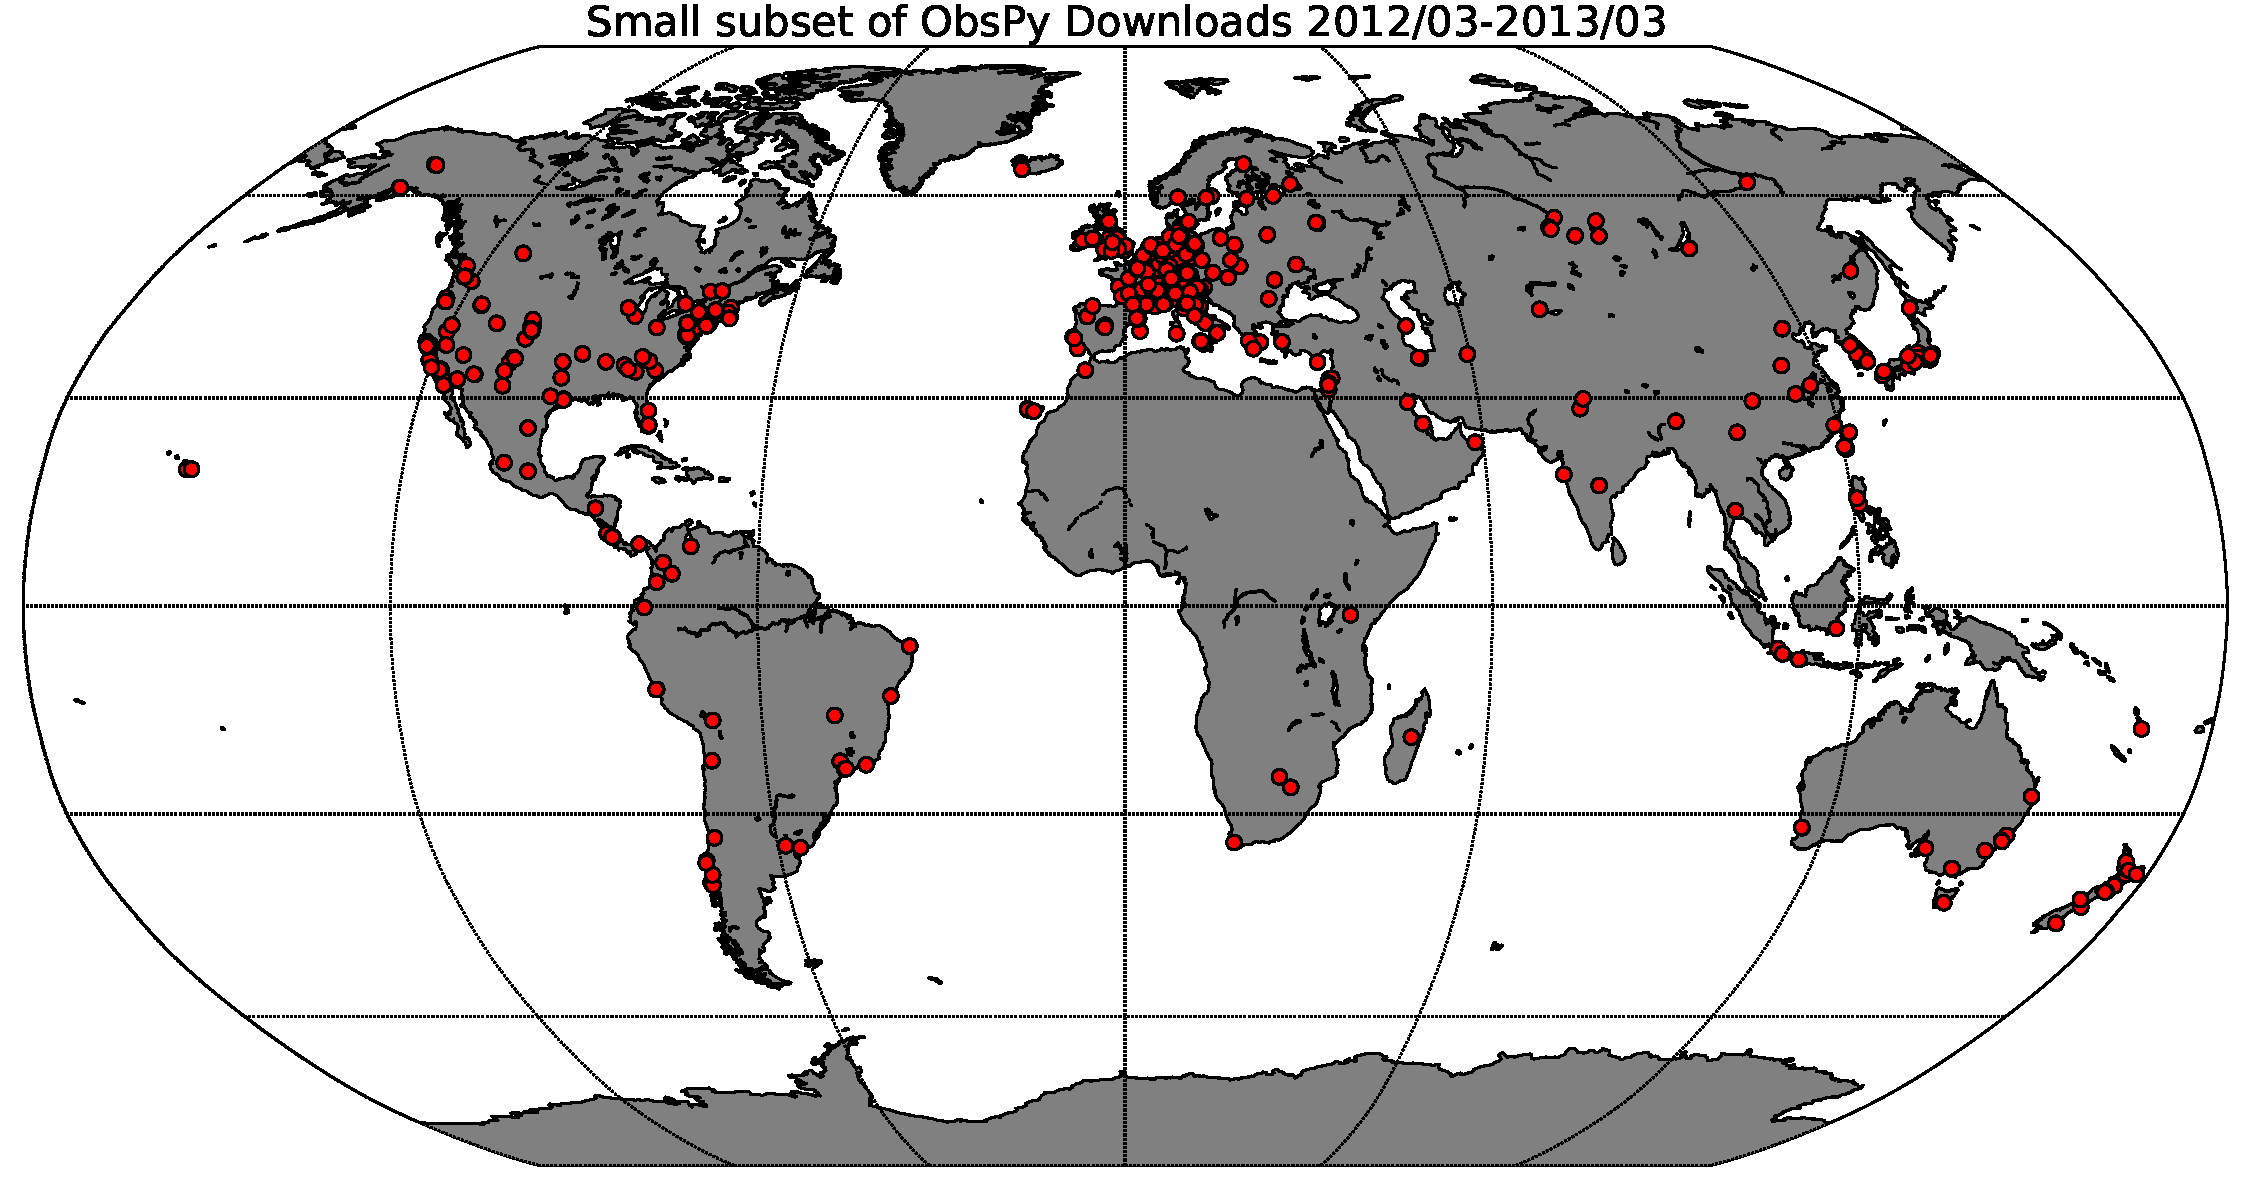
\includegraphics[width=0.90\columnwidth]{./Scripts/ObsPyUsers.pdf} \\
    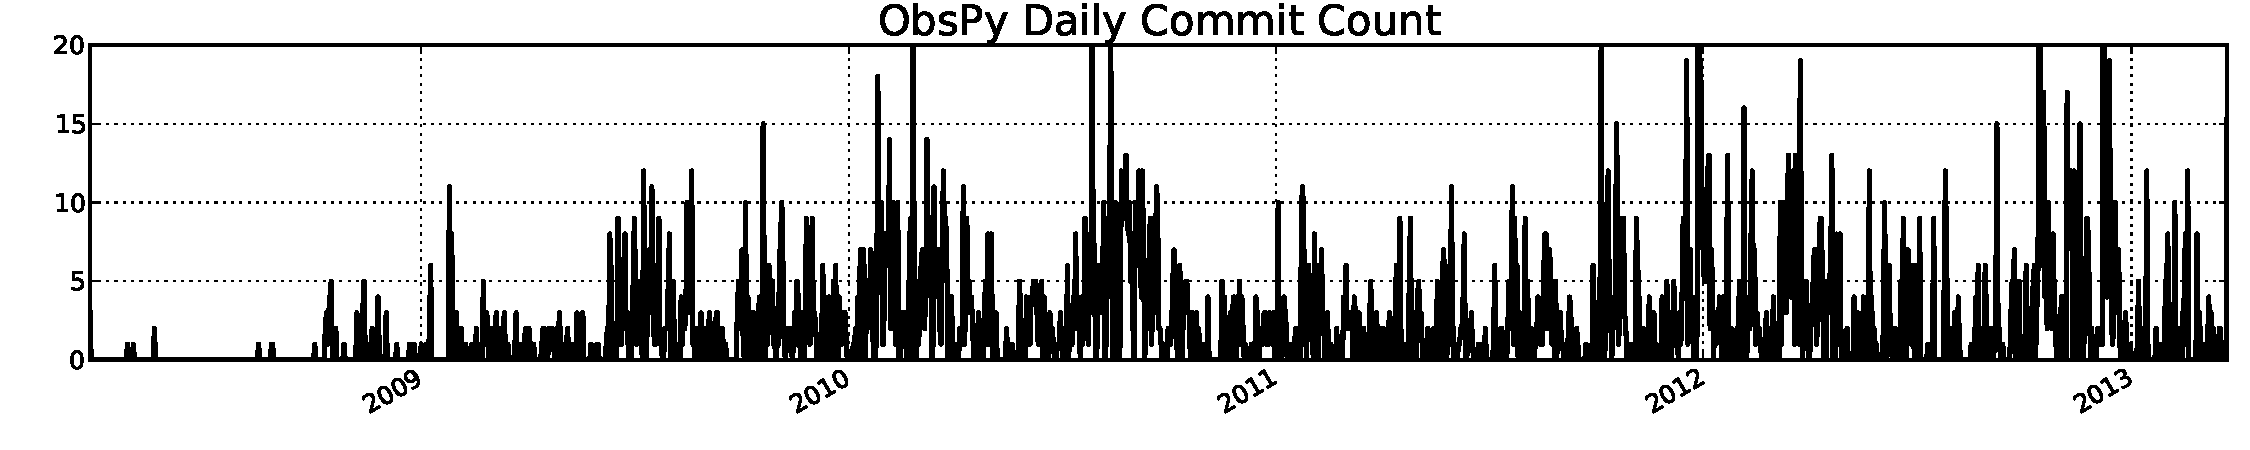
\includegraphics[width=0.90\columnwidth]{./Scripts/ObsPyDailyCommits.pdf} \\
    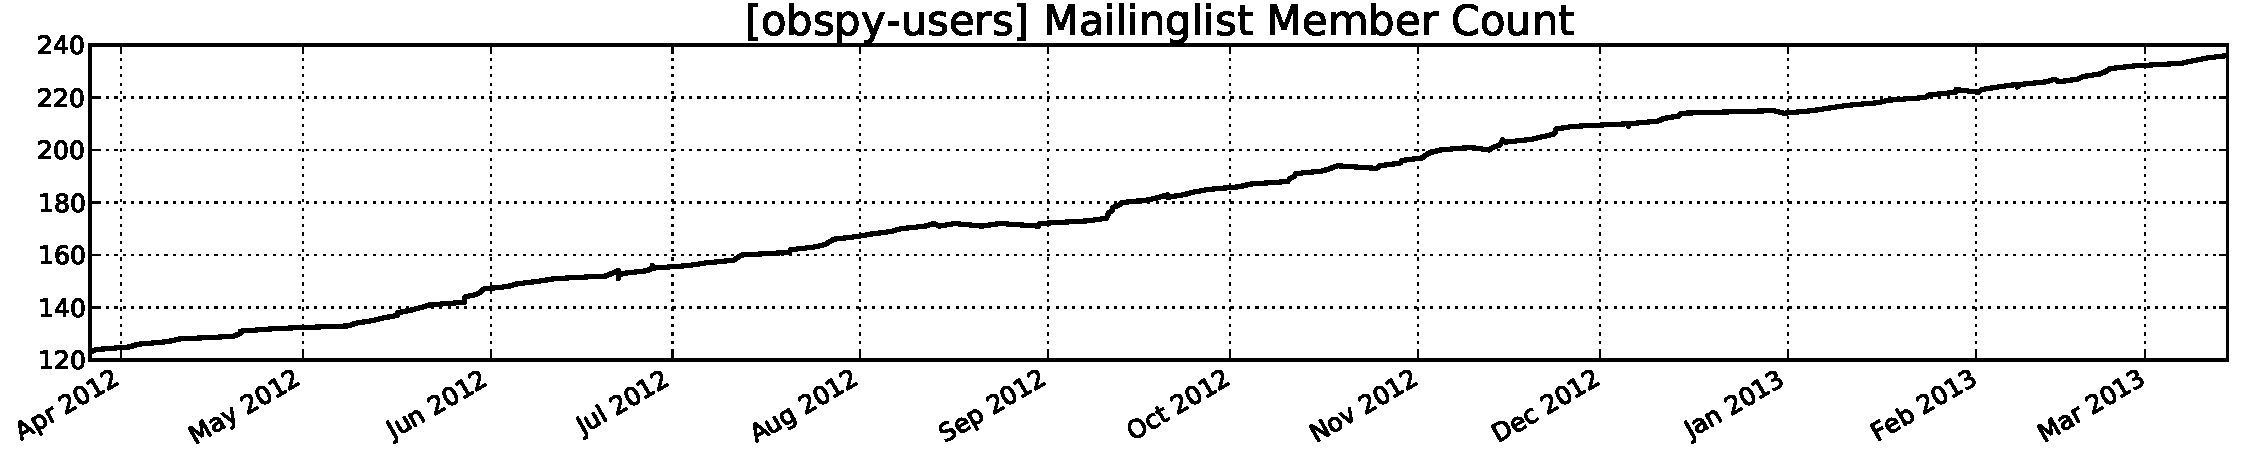
\includegraphics[width=0.90\columnwidth]{./Scripts/ObspyMailinglist.pdf}
\end{center}
}
\vspace{\MyBoxVSep}


\MyBox[8em]{
%\section*{Outlook}
\section*{http://www.obspy.org}
\begin{itemize}
    \item Source Code, Bug Tracker, and Wiki
    \item Extensive documentation and example gallery
    \item Tutorial on how to get started
    \item \textbf{[obspy-users]} mailing list
    \item Installation Instructions for various platforms
    \item Use cases
\end{itemize}
}
\vspace{\MyBoxVSep}



\MyBox[1em]{
\section*{References}
\small
B\textsc{eyreuther}, M., R. B\textsc{arsch}, L. K\textsc{rischer}, T. M\textsc{egies}, Y. B\textsc{ehr} and J. W\textsc{assermann} (2010)\\
\textbf{ObsPy: A Python Toolbox for Seismology}\\
Seismological Research Letters, 81(3):530-533, doi:10.1785/​gssrl.81.3.530\\

M\textsc{egies}, T., M. B\textsc{eyreuther}, R. B\textsc{arsch}, L. K\textsc{rischer} and J. W\textsc{assermann} (2011)\\
\textbf{ObsPy – What can it do for data centers and observatories?}\\
Annals Of Geophysics, 54(1), 47-58, doi:10.4401/ag-4838
\vspace{2.805ex}
}\vspace{\MyBoxVSep}


\end{multicols}


\end{document}
